\chapter{Methodology}
This chapter describes the data collection of merge samples, and the empirical evaluation of the intentions language and intention-based variant integration tool BACONTOOL.

\section{Data collection}
Two methods for collecting data from open-source ecosystems have been used, one for gathering a ground truth for how variant integration is achieved through merging, and one for procuring variants for hypothetical but realistic \todo{realistic or authentic?} integration scenarios. We denote the output of the former method \textit{merge examples} and the output of the latter method \textit{integration scenarios}. The merge examples are used for understanding the context and execution of the variant-integrating merge. They can also be replayed for validation, since they represent the ground truth outcome of the two merge parents. As such, the merge examples serve as an important validation tool. However, since the merge examples are extracted from a three-way merging tool, they are disadvantageous for replaying in BACONTOOL, since three-way information is not available in that environment. To this end, we use the integration scenarios, which are free from three-way contamination, but are instead taken out of their context.

\subsection{Collecting ground truth merge examples}
To identify and validate the integration intentions we analyze variant-related merges and extract common patterns. We begin by retrieving all merges, and discard those that merged cleanly, thereby retaining those that merged with conflicts. Merged with conflicts signifies a syntactic conflict which is an indicator of potential feature integration. In order to investigate further, for each of these merges, we save the entire source tree as it was 
a) after the merge, i.e. the \textit{result},
b) in the first parent, i.e. the \textit{base}\todo{Change terminology to avoid confusion with git merge-base}, and
c) in the second parent, the \textit{remote}. We call this triple of source trees the \textit{related artifacts} of the merge, the relationship between its parts is shown in Figure \ref{intentions:mergespace}. Retaining and inspecting the source trees of the parents allows for insights to be gathered, and in particular the ability to replay the merge in order to reach the known result. Note that the search space, the entire set of merges encompasses \textit{all} merges, that is, merges that occurred in a fork but were subsequently merged into the mainline are also included. We do \textit{not} use the \texttt{-{}-first-parent} option to Git, which would discard such further merges residing in recursive parents, and instead use only the first parent when finding merges. The merges that are included by this broader search scope originate either from ordinary feature merging or from pull requests where the branch of the requester is out of date.%\todo{Figure showing ABL feature integration and Deltabot feature integration.}

When the related artifacts from each merge have been collected, we inspect them and discard merges with any of the following properties: 
a) all conflicts occurred in non-source-code artifacts, b) at least one artifact cannot be compiled, c) there are only whitespace changes between the merge parents, or d) contain some project-specific uninteresting changes (see Results for examples of uninteresting in practice).

\begin{figure}[h]
    \centering
    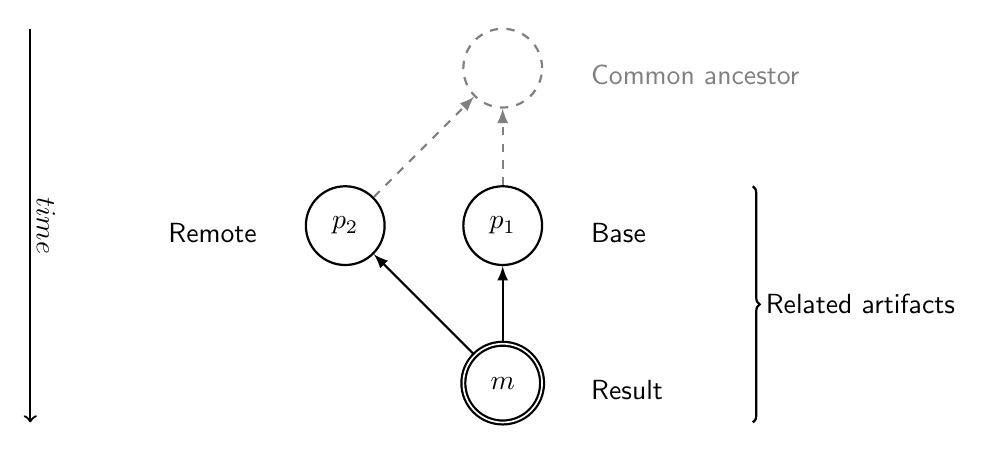
\begin{tikzpicture}
        \tikzset{every node/.append style={font=\sffamily}}
        \tikzstyle{linez} = [thick]
        \tikzstyle{commit} = [shape=circle,draw=black, minimum size=1cm, linez]
        \tikzstyle{ancestor} = [draw=gray, dashed]
        \tikzstyle{messager} = [xshift=1cm, yshift=-0.6cm, anchor=west]
        \tikzstyle{messagel} = [xshift=-1cm, yshift=-0.6cm, anchor=east]
    
        \node[commit, double, label={[messager]Result}] (res) at (0,0) {$m$};
        \node[commit, label={[messager]Base}] (ba) at (0,2) {$p_1$};
        \node[commit, label={[messagel]Remote}] (re) at (-2,2) {$p_2$};
        \node[commit, ancestor, label={[messager, color=gray]Common ancestor}] (an) at (0,4) {};
        
        \draw[thick, decoration={brace,mirror,raise=5pt},decorate] (3,-0.5) -- node[right=6pt] {Related artifacts} (3, 2.5);
        
        \draw[thick,->] (-6,4.5) to node[pos=0.5, xshift=0.2cm, rotate=-90] {$time$} (-6,-0.5);
        
        \draw [->, -latex, linez] (res) -- (ba);
        \draw [->, -latex, linez] (res) -- (re);
        \draw [->, -latex, ancestor, linez] (re) -- (an);
        \draw [->, -latex, ancestor, linez] (ba) -- (an);
        % NOTE: There is a bug in tikz with -latex arrows and colors. The arrows should therefore be drawn last, otherwise the colors of the arrowheads can mess up.
        
    \end{tikzpicture}
    \caption{Merge commit context. The merge commit $m$ has two parents, $p_1$ and $p_2$. The entire state of the source tree is gathered, as they appear in these commits, denoted \textit{result}, \textit{base}, and \textit{remote}. This triple of source tree sets constitute the \textit{related artifacts} of the commit $m$.}
    \label{intentions:mergespace}
\end{figure}

\subsection{Creating authentic merging tasks}
We select a number of forks that have some \textit{interesting} changes \cite{stanciulescu2015}. It does not matter whether they are still actively maintained or not, because we set the scenario at the \head of the fork, and then compare with either a) the latest common ancestor commit \texttt{\#ancestor} in fork and mainline, or b) an arbitrary number of commits after \texttt{\#ancestor} in the mainline. We create scenarios by partially replaying conflict merges, based on their variability-related diffs.

Done on Marlin + BusyBox + Vim.

\section{Internal evaluation}
We both replay merge examples and merge authentic scenarios. Each participant receives a task, and performs it in both Eclipse CDT and BACONTOOL. The number of actions for each task in each editor is saved for analysis, as is the resulting output file. Each tasks consists of a number of input files from the two variants being integrated, together with a textual description of what the integration goal is.

\section{Controlled experiment}
This sections desrcibes the experimental design and setup.
%Designed based on Melo et al \cite{melo2016latin} (also the subsequent paper from 2017). % -- it has really good related work that can be used to show that the preprocessor (and configurations) are often erroneous.

\subsection{Objective}
To establish the beneficence of of the intention-based approach in general, and the intention-based integration tool in particular, we evaluate the tool using subject programs from other sources than Marlin, since Marlin was used to elicit the intentions. The purpose of this controlled experiment is to answer the following research questions:
\begin{enumerate}[label={Q\arabic*}]
    \setcounter{enumi}{1}
    \item \RQB
    \item \RQC
\end{enumerate}

\subsection{Treatments}
In order to study the beneficence of our intention-based approach, we let each participant solve one task using an ordinary unstructured merge tool, and one task using BACONTOOL. The two treatment levels are thus \textit{unstructured merging tool} \texttt{UNS} and \textit{Incline-bacon} \texttt{MPS}.

\subsection{Subjects}
We prepare two programs to be used in the experiment, using the process for collecting authentic variant integration scenarios, \po, based on \busybox, and \pt, based on \vim. These two programs are created as condensed versions of the changeset of a particular fork variant, for brevity and comprehension during the experiment. Table \ref{method:charac} lists the characteristics of the subject programs. \textit{Chunks and excluded chunks} shows the number of selected chunks from the full changeset to be in the program, and the excluded count. \textit{Average Included (Excluded) Chunk Length} (AICL/AECL) is the average length of each included chunk and excluded chunk. This should be understood as selecting the most suited changes across the files, and placing them in a single file, in order to not waste valuable time for the participants on long blocks without any changes, as to keep the programs brief.

(LOC might not be applicable, since we have two input files)

We choose \busybox~ and \vim~ as representative subjects because they are highly-configurable open source systems, and have been subjects in previous studies \cite{berger2013study}, \cite{liebig2010preprocessor}, \cite{liebig2011discipline}.

\begin{table}[h]
    \centering
    \caption{Characteristics of the tasks \po~and \pt.}
    \label{method:charac}
    \begin{tabular}{c l c c c c c}
    \hline
    \hline
        \textbf{Prg} & \textbf{Origin} & \textbf{LOC} & \textbf{\#chunks} & \textbf{AICL} & \textbf{\#excl. chunks} & \textbf{AECL} \\\hline
        \po & \busybox & - & - & - & - & -\\\hline
        \pt & \vim & - & - & - & - & - \\
        \hline
        \hline
    \end{tabular}
\end{table}

\subsection{Design}
The experiment is a 2$\times$2 \textit{within-subjects} Latin square design \cite{box}. Each developer performs two tasks with the treatment order and program order randomized in order to reduce learning effects. Table \ref{method:ls1} shows the base Latin square.
Since developers are assigned at random, no further permutation of the treatments in the 2$\times$2 Latin square is required, since the two other possible combinations would be redundant with respect to program order and treatment.

\begin{table}[h]
\centering
\caption{Latin Square (2$\times$2).}
\label{method:ls1}
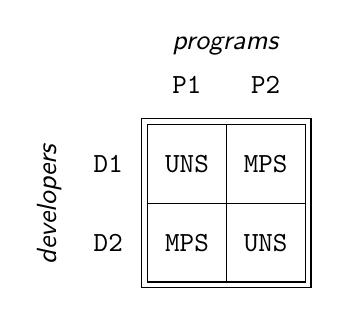
\begin{tikzpicture}
    \node[minimum size=1cm,draw=black] (sba) at (0,0) {\texttt{MPS}};
    \node[minimum size=1cm,draw=black] (sbb) at (1,0) {\texttt{UNS}};
    \node[minimum size=1cm,draw=black] (saa) at (0,1) {\texttt{UNS}};
    \node[minimum size=1cm,draw=black] (sab) at (1,1) {\texttt{MPS}};
    \node[minimum size=1cm] (ld1) at (-1,1) {\texttt{D1}};
    \node[minimum size=1cm] (ld2) at (-1,0) {\texttt{D2}};
    \node[minimum size=1cm] (lp1) at (0,2) {\texttt{P1}};
    \node[minimum size=1cm] (lp2) at (1,2) {\texttt{P2}};
    
    \node[minimum size=2.15cm,draw=black] (square) at (0.5,0.5) {};
    \node[] (lprog) at (0.5, 2.5) {\textit{programs}};
    \node[rotate=90] (ldevs) at (-1.75, 0.5) {\textit{developers}};
\end{tikzpicture}
\end{table}

\subsection{Execution}
Before running the actual experiment, we executed a pilot study with the authors of \cite{lillack2017intentions}, in order to assess the presentation of the tasks and the distribution of our tooling.

Planned execution with subjects:
\begin{itemize}
    \item Introduction/tutorial to both tools
    \item Small warm-up example
    \item Distribution of tasks
    \item Execution
    \item Debriefing interview + questionnaire
\end{itemize}